{\titlespacing*{\chapter}
{0pt}{-5pt}{-5pt}\chapter[Summary]{}}
\rule{\linewidth}{0.5mm}
\hspace*{0pt}
\section*{Design of a machine learning algorithm for restaurant \\recommendations based on labeled and textual data}
\rule{\linewidth}{0.5mm}

\textbf{Students:}
\hfill
\textbf{Supervisors:} \\
Arnoud De Jonge
\hfill
prof. dr. ir. Toon De Pessemier \\
Arno Vermote
\hfill
prof. dr. ir. Luc Martens \\
\\
\hspace*{0pt}\hfill Master Computer Science


\begin{otherlanguage}{english}
\begin{multicols}{2}
[
\section*{\centering Abstract}
Recommender systems provide assistance to end users in making decisions. Existing state-of-the-art algorithms use either labeled or textual data. We combined both data sources to increase the accuracy of the predicted scores. On the Yelp Dataset we measured an RMSE of 1.1107, which is better than the Wide \& Deep Learning RMSE of 1.4025 and the DeepCoNN RMSE of 1.1642. Predicting reviews of 1/5 stars or 5/5 stars remains a problem, due to the limited training samples of these classes. 
]

\section*{1. Introduction}
Recommender systems are used by many service providers and webshops to provide a smart filtering of items. Often, these recommendations are personalised to match the preferences of the users. This is done by collecting data for every user and aggregating this into user profiles. Similarly, all data of each item is aggregated into an item profile. Then, these profiles are compared to identify if the item matches the preferences of the user.

The state of the art consists of DeepCoNN \cite{deepconn_eng_summary} for recommendations based on purely textual data. This will often be written reviews from customers. The state of the art for recommendations based on labeled data is Wide \& Deep Learning \cite{wide_deep_learning_paper_eng_summary}.\newline
In this paper we explore the potential performance gains when utilizing both data sources to predict the score a specified user gives to a specified item. The domain of the predicitons will be scores for restaurants. The data is sourced from Yelp. \cite{Yelp_Dataset_eng_summary}

\section*{2. Methodologies}
We will first transform the textual data into user- and item profiles using Natural Language Processing (NLP) techniques. Then, these profiles will be combined with profiles created using the labeled data. The result will be fed into a neural network, which will make a prediction for the expected score of that user for that restaurant.

\subsection*{Labeled Data Profiles}
These profiles are constructed using the labels available in the Yelp dataset. This dataset assigns each restaurant a collection of \q{categories} and \q{attributes}. These labels are then one-hot encoded in a vector, which represents the restaurant profile. The user profiles are then constructed using a sum for each label of the rated restaurants, multiplied by their normalized score minus 0.5 (neutral score after normalization). This way we model the user profile with the same labels as the restaurant profiles, but with the user's preference included.

\subsection*{Profiles From Text}
We create a second pair of profiles, but now using the written reviews as data source. For this, we will use BERTopic. \cite{bertopic_paper_eng_summary} This is mainly an offline algorithm, but online and other variations exist. BERTopic's structure consists of multiple parts: each part can be swapped out individually for another similar method. As a result of this, the algorithm is highly customizable. Therefore constructing an adaptation is almost trivial. The first part is the embeddingsmodel. This will convert the sentences into numeric vectors. For the embeddingsmodel we will use transformer models, a relatively new discovery in NLP. To be precise, we are using Sentence-BERT \cite{sentence_bert_eng_summary}. \newline
After generating a numeric vector for each sentence, a dimensionality reduction algorithm reduces the dimension of that vector. This will be done to tackle the challenges that comes with high-dimensional data \cite{curse_of_dim_eng_summary}. Any dimensionality reduction algorithm such as UMAP or PCA can be used. For the online variant we chose an adaptation to PCA, namely Incremental PCA \cite{ipca_eng_summary}.\newline
After the dimension is reduced, the algorithm will produce a clustering. Once again multiple clustering algorithms can be used, including HDBSCAN and K-Means. In our experiments we utilize MiniBatch K-Means \cite{kmeans_minibatch_eng_summary} for the online variant. \newline
The final step is to construct a representation for every cluster. This is done by creating a bag-of-words representation for the combined text of all documents in one cluster. Afterwards c-TF-IDF \cite{bertopic_c_tf_idf_eng_summary} is applied. This is a class based variant of TF-IDF. The final representation of one cluster or topic consists of the most frequent words defined by c-TF-IDF. It is possible to finetune these representations even more, for example by using KeyBERT \cite{keybert_eng_summary}.

\subsection*{Creating Predictions}
A neural network is a class of supervised machine learning models. It is inspired by the way a human brain works, with neurons connected to each other in layers. Often, neural networks have the most potential to achieve the lowest loss of all machine learning methods after extensive training. \cite{cursus_ML_supervised_eng_summary} Neural networks have the downside that it is difficult to interpret or explain the decision making process.\newline
The combined input data as calculated in the previous steps is provided to a neural network, with all profiles for one specific restaurant and one specific user at a time. The neural network then provides a score, wich corresponds to the predicted rating which the user would give to that restaurant.

\section*{3. Experimental Setup}
\subsection*{BERTopic}
To use textual reviews in a neural network, we must convert these into a numeric inputvector. We focus on the added value of the topic modelling algorithm BERTopic. The model takes multiple textual documents as input to generate a clustering. Each cluster is then represented by a set of words. 

In our case we use the sentences from the reviews as input for the BERTopic model. Given the large amount of reviews, we expect to reach the limitations of system memory using the standard BERTopic algorithm. Consequently, we investigate the performance of a better scaling online BERTopic variant. Using various BERTopic models, we can manufacture the profiles of users and restaurants. This is done for every user and restaurant based on the reviews they gave or received. We evaluate the different building blocks to implement a BERTopic model: we will compare the profiles that are based on the clustering of a model, to profiles created by solely using the representations. Another interesting hyperparamter is the amount of clusters, which is equivalent to the length of the final profiles. Finally we will measure the impact of using subjective predefined topics to assist the model training. Note that in this last experiment, the model is free to adapt or dismiss inaccurate topics.

Additionally we experiment with sentiment analysis \cite{sentiment_transformer_paper_eng_summary}, which works independently from the BERTopic algorithm. Sentiment analysis is used to extract positive or negative user experiences from a written review without any additional information. Reviews can contain positive and negative feedback at the same time. Combining this with BERTopic to determine the subject can result in an improved feature vector.

To evaluate the results we will use a neural network. This will be a simple neural network with 5 hidden layers. To compare different profiles, all other parameters remain fixed. The combination of profiles that provides the minimal loss will be considered better. Since a neural network is a detour to evaluate a BERTopic model, we also use an alternative method: to directly evaluate the clustering we make use of clustering metrics such as the silhouette index or Davies-Bouldin index. Finally we analyse if the same patterns occur between the clustering metrics and the loss.


\subsection*{Neural Network}
After the best performing combination of input profiles is found as explained in the previous sections, we try to adapt the neural network to further enhance its predictive capabilities. We experiment with multiple parameters to create an optimal neural network architecture, based on the general performance, measured in MSE. After finding the ideal model using the MSE criterium, edge case performance and rigidity of the network is tested. We treat each parameter as fully independent to all other parameters. This assumption is not entirely sound, but conducting a full grid search for every combination of parameters would be too computationally expensive. While this assumption might not provide us with the overall best possible network, it will likely suffice for all practical purposes.

We explore the amount of layers in the neural network: we implement different networks from one up to eight hidden layers. Each hidden layer halves the amount of neurons. The final output layer has one neuron. The models with five or more hidden layers have a small adaptation, where they will first increase the amount of neurons up to 150\% of the amount of neurons in the input vector, to then scale down gradually to one neuron in the output layer.\newline
We also experiment with the more dynamic ADAGRAD optimizer, compared to the basic SGD optimizer. After finding the best performing network configuration, we measure the effect of the size of the dataset on the performance and the effect of the cold start problem on the ability to provide accurate predictions.\newline
To validate the performance comes from combining the textual and labeled data sources, we also trained a Random Forest model with this data. We then compare our final results to other algorithms: traditional implementations as state-of-the-art techniques.


\section*{4. Results and Discussion}
\subsection*{NLP profiles}
We can conclude that an online BERTopic model heavily outperforms the offline standard. We did not discover any significant differences when comparing profiles based on clustering against the profiles based on the representation. Also, the addition of predefined topics yields similar results. When increasing the amount of clusters from 50 to 400 we see a marginal increase in performance, yet not any remarkable improvements. The addition of sentiment does significantly increase the performance. The top performance is gained when only applying sentiment to restaurant profiles. \newline
Finally, we observe a correlation in the loss and results of the clusteringmetrics. This means that it is possible to determine if a BERTopic model has an acceptable clustering without training a neural network. Note that these metrics can be influenced when using higher dimensions without having the same impact on the loss. In addition, metrics are not applicable to NLP analyses that are independent from BERTopic, e.g.: sentiment analysis.


\subsection*{Rating Predicions}
As discovered in the previous section, the input parameter will consist of two NLP profiles with each a dimension of 400, combined with two profiles extracted from the labeled dataset. In total, the inputvector has a dimension of $1000$. The optimal network architecture to handle this input exists of six hidden layers, but networks with seven or eight hidden layers also perform well.\newline
SGD was not able to sufficiently train the network. The use of the ADAGRAD optimizer is necessary. A learning rate of 0.0002 seemed optimal. The network could be sufficiently trained and tested with only 50\% of the data set. With even smaller data sets, the model would start to sacrifice generality.\newline
The effect of the cold start problem is limited. For users with less than five reviews we were able to predict ratings with an accuracy of 22\%, compared to an accuracy of 36\% for users with more than 25 reviews. However, we noticed the network really struggles to predict the less represented classes. We measured an accuracy of only 1.7\% for 1-star reviews (\autoref{fig:eng_summ_acc_1star}). This is because the network tends to fall back to predicting 4 stars when it is uncertain, since this value provides a middle ground. We believe further research into this problem is required.

Finally, we were able to beat both DeepCoNN and Wide \& Deep Learning in terms of RMSE (\autoref{fig:eng_summ_RMSE}). The RMSE represents the average difference between the provided score by the user and the predicted score (out of 5 stars). This confirms our hypthesis that the combination of multiple data sources can lead to better predictions.

\begin{figure}[H]
    \begin{center}
        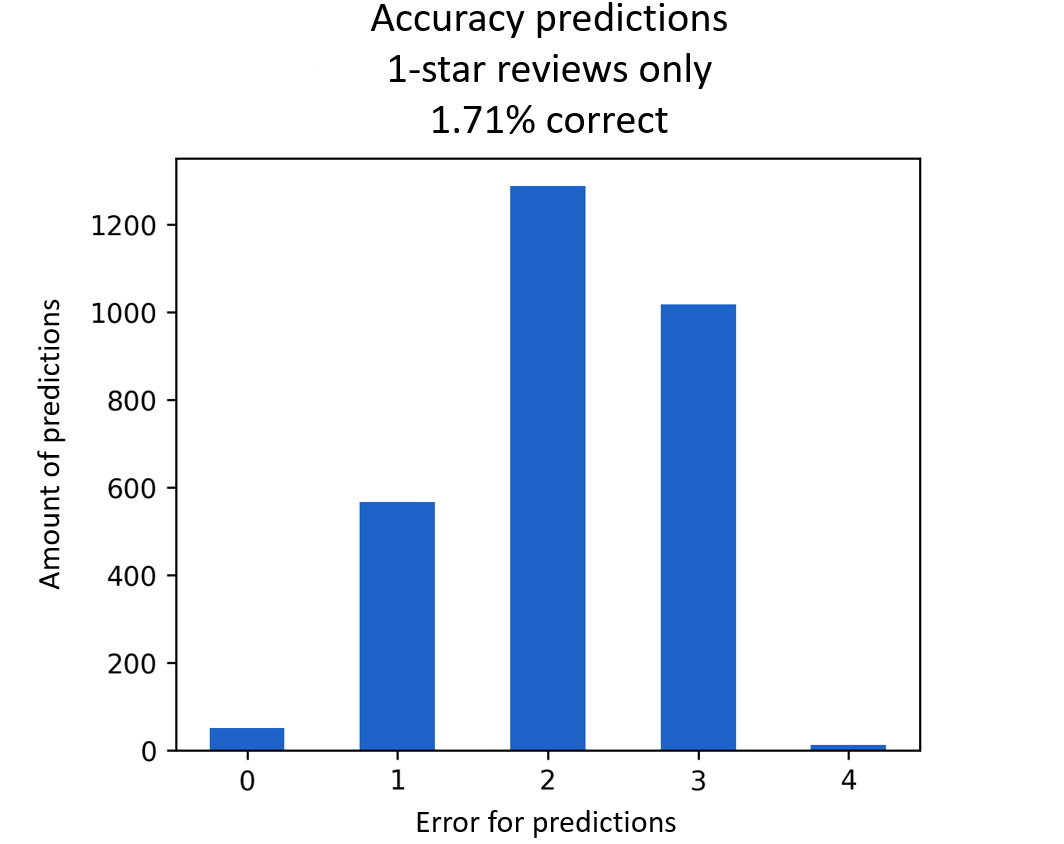
\includegraphics[width=8cm]{fig/eng_summary/accuracy_1star.png}
    \end{center}
    \caption{Prediction Accuracy of 1-star Reviews}
    \label{fig:eng_summ_acc_1star}
\end{figure}

\begin{figure}[H]
    \begin{center}
        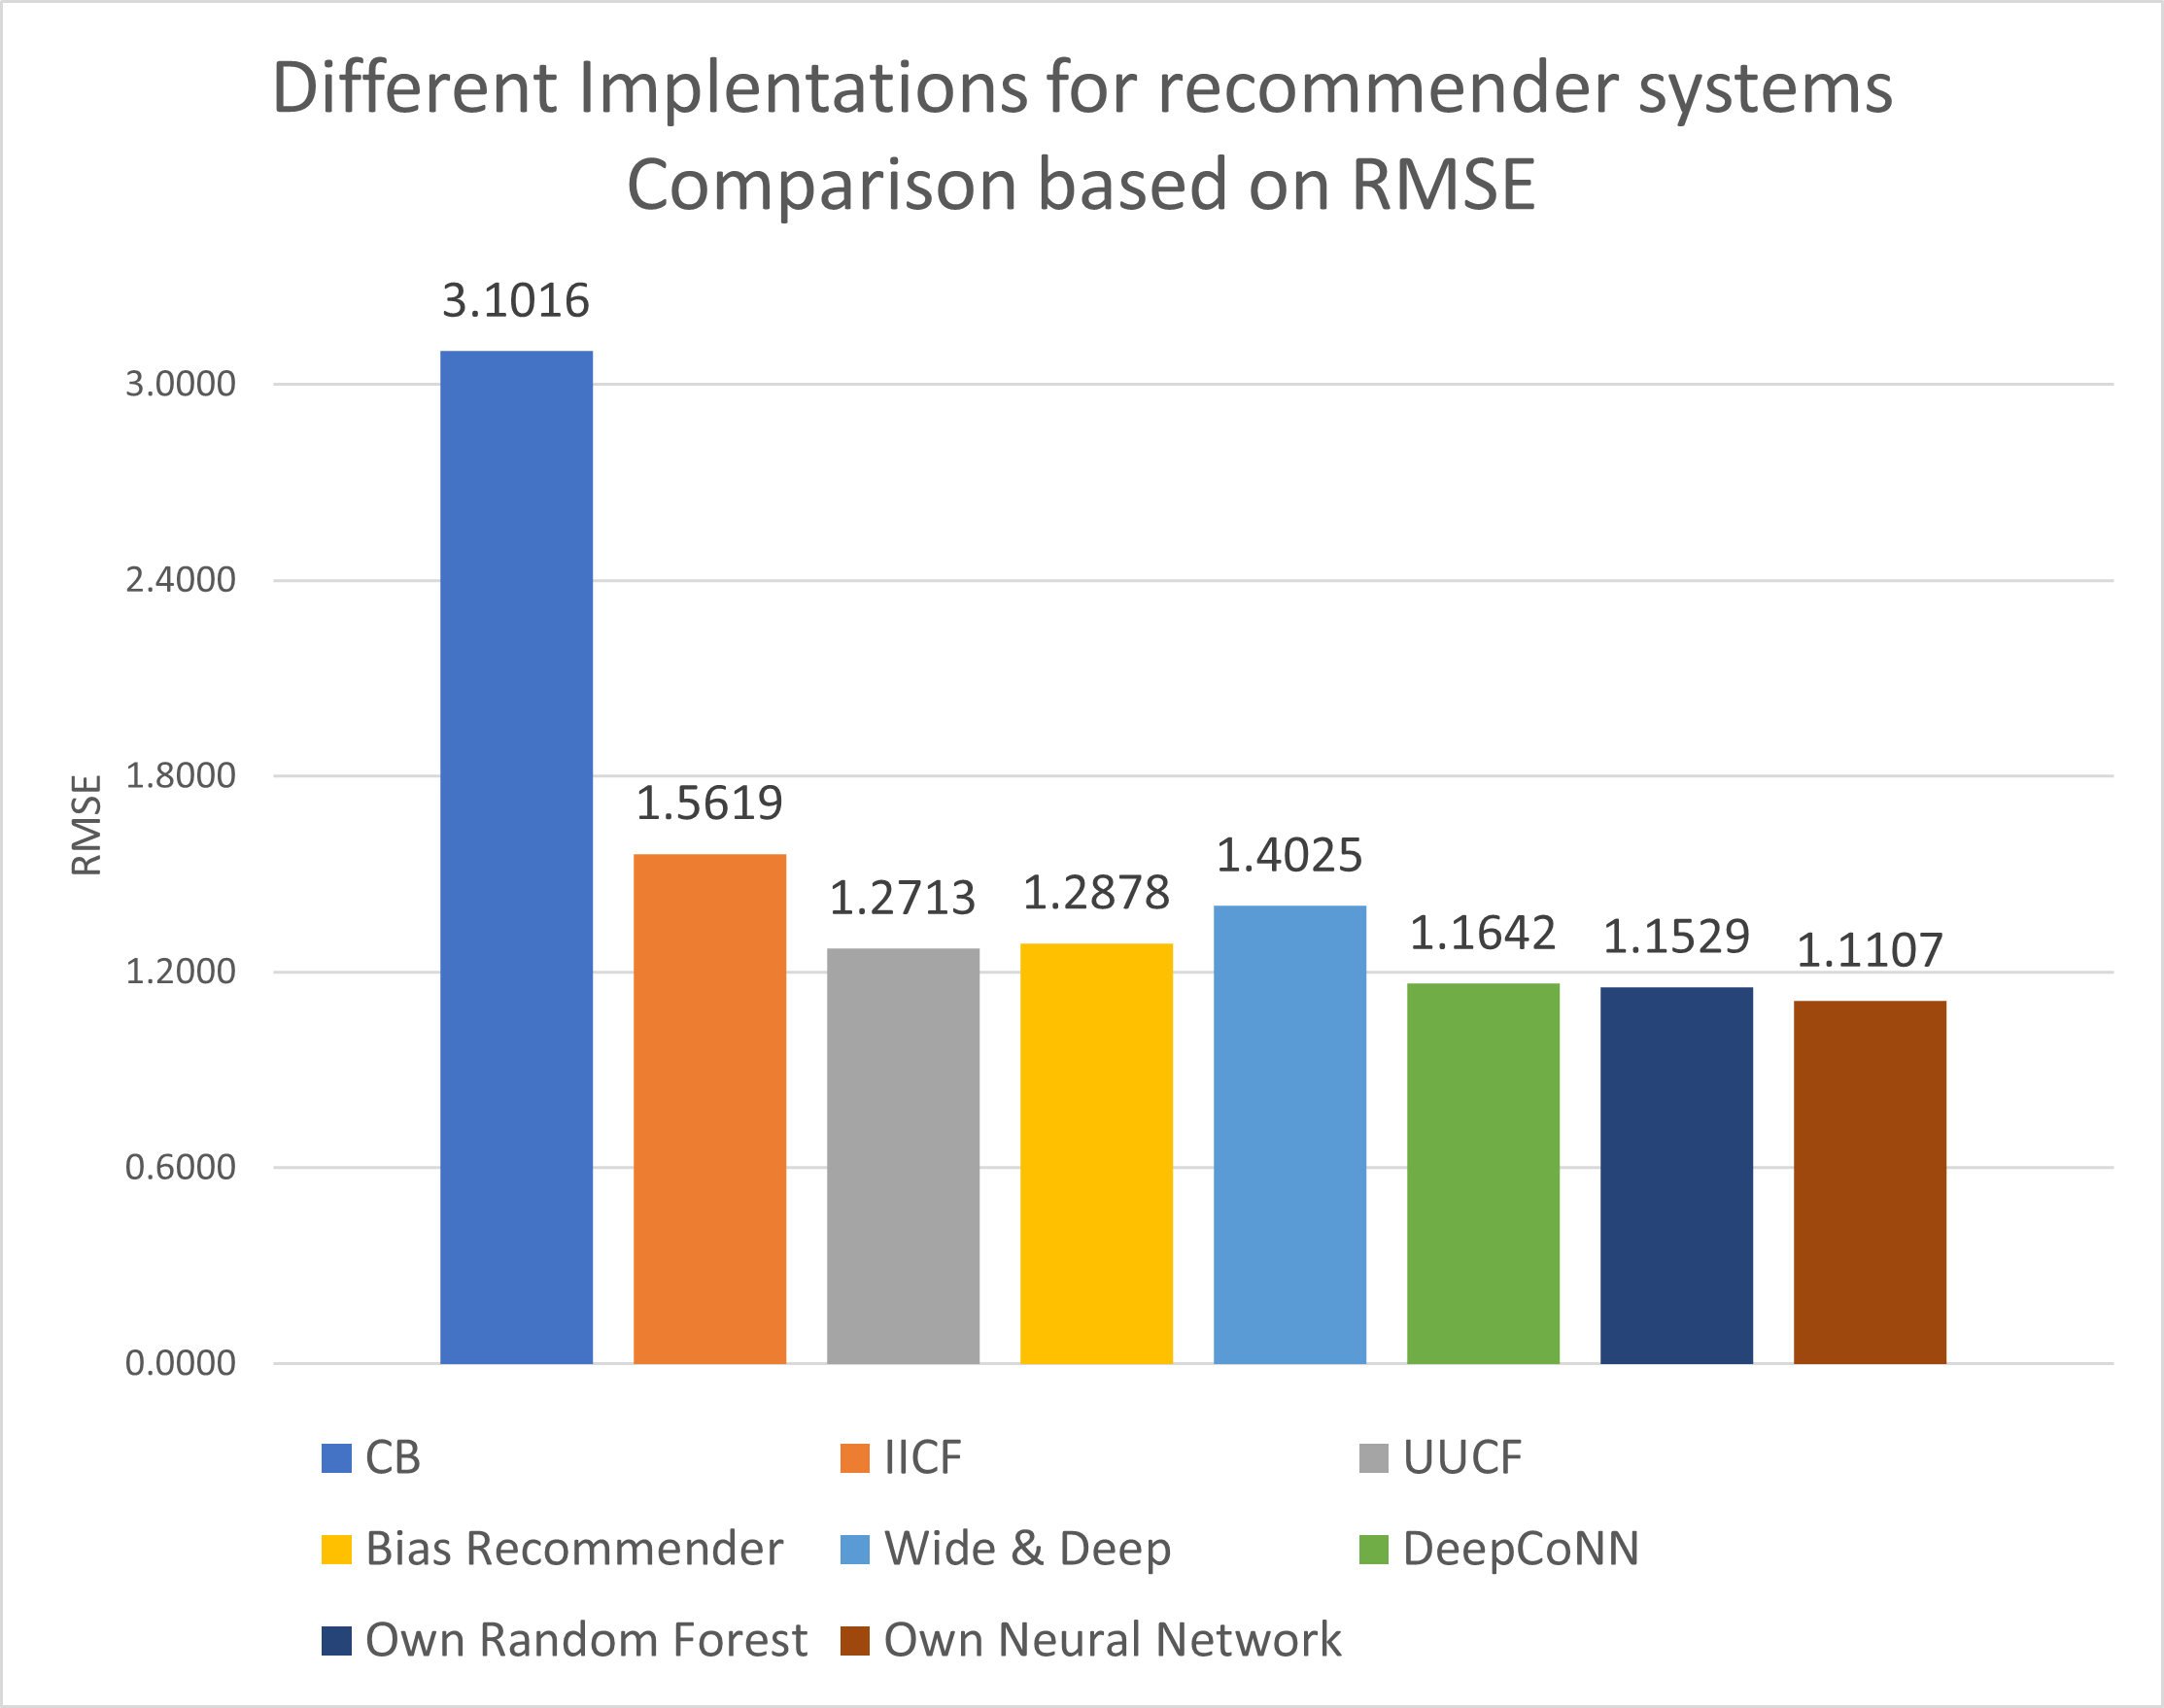
\includegraphics[width=8cm]{fig/eng_summary/comparison_implementations.png}
    \end{center}
    \caption{Comparing of RMSE for different implementations \cite{deepconn_eng_summary, wide_deep_learning_paper_eng_summary}}
    \label{fig:eng_summ_RMSE}
\end{figure}

\printbibliography[heading=subbibliography, keyword={eng_summary}]
\end{multicols}
\end{otherlanguage}
